% !TEX TS-program = pdflatex
% !TEX encoding = UTF-8 Unicode

% This is a simple template for a LaTeX document using the "article" class.
% See "book", "report", "letter" for other types of document.

\documentclass[11pt]{article} % use larger type; default would be 10pt.
\setcounter{secnumdepth}{2}

\usepackage{paralist} % very flexible & customisable lists (eg. enumerate/itemize, etc.)

\usepackage[utf8]{inputenc} % set input encoding (not needed with XeLaTeX)
\usepackage{float} % to place float images correctly
\usepackage{color} % to color text
\usepackage{enumitem} % for lists
\usepackage{subfigure} % for mockups
\usepackage[font={it}]{caption} % for captions
\usepackage{censor}
%%% Examples of Article customizations
% These packages are optional, depending whether you want the features they provide.
% See the LaTeX Companion or other references for full information.

%%% PAGE DIMENSIONS
\usepackage{geometry} % to change the page dimensions
\geometry{a4paper} % or letterpaper (US) or a5paper or....
% \geometry{margin=2in} % for example, change the margins to 2 inches all round
% \geometry{landscape} % set up the page for landscape
%   read geometry.pdf for detailed page layout information

\usepackage{graphicx} % support the \includegraphics command and options

% \usepackage[parfill]{parskip} % Activate to begin paragraphs with an empty line rather than an indent

\usepackage{listings}
\usepackage{color}
 
\definecolor{codegreen}{rgb}{0,0.4,0}
\definecolor{codegray}{rgb}{0.5,0.5,0.5}
\definecolor{codepurple}{rgb}{0.58,0,0.82}
 
\lstdefinestyle{mystyle}{ 
    commentstyle=\color{magenta},
    keywordstyle=\color{blue}\bfseries,
    numberstyle=\tiny\color{codegray},
    stringstyle=\color{codepurple},
    basicstyle=\footnotesize,
    breakatwhitespace=false,         
    breaklines=true,                 
    captionpos=b,                    
    keepspaces=true,                 
    numbers=left,                    
    numbersep=5pt,                  
    showspaces=false,                
    showstringspaces=false,
    showtabs=false,                  
    tabsize=2,
   emph={self}, 
   emphstyle=\color{blue}, 
   emph={[2] BookingManager, FineManager}, 
   emphstyle=[2]\color{codegreen}\bfseries, 
   emph={[3]__init__, newBook, removeReservation, getReservation, manageExpired, min_heap, pop, now, timedelta, expireReservation}, 
   emphstyle=[3]\color{codegreen}, 
}
 
\lstset{style=mystyle}





%%% PACKAGES
\usepackage{booktabs} % for much better looking tables
\usepackage{array} % for better arrays (eg matrices) in maths
%\usepackage{paralist} % very flexible & customisable lists (eg. enumerate/itemize, etc.)
\usepackage{verbatim} % adds environment for commenting out blocks of text & for better verbatim
\usepackage{subfig} % make it possible to include more than one captioned figure/table in a single float
% These packages are all incorporated in the memoir class to one degree or another...

%%% HEADERS & FOOTERS
\usepackage{fancyhdr} % This should be set AFTER setting up the page geometry
\pagestyle{fancy} % options: empty , plain , fancy
\renewcommand{\headrulewidth}{0pt} % customise the layout...
\lhead{}\chead{}\rhead{}
\lfoot{}\cfoot{\thepage}\rfoot{}

%%% SECTION TITLE APPEARANCE
\usepackage{sectsty}
\allsectionsfont{\sffamily\mdseries\upshape} % (See the fntguide.pdf for font help)
% (This matches ConTeXt defaults)

%%% ToC (table of contents) APPEARANCE
\usepackage[nottoc,notlof,notlot]{tocbibind} % Put the bibliography in the ToC
\usepackage[titles,subfigure]{tocloft} % Alter the style of the Table of Contents
\renewcommand{\cftsecfont}{\rmfamily\mdseries\upshape}
\renewcommand{\cftsecpagefont}{\rmfamily\mdseries\upshape} % No bold!

\newcommand{\pe}{PowerEnJoy }
\newcommand{\pecomma}{PowerEnJoy, }
\newcommand{\bul}[1]{\indent$\bullet$ #1\\}

\usepackage{listings}
\usepackage{pxfonts}
%%% END Article customizations

%%% The "real" document content comes below...




\title{Design Document}
\author{Simone Mosciatti \& Sara Zanzottera}

\begin{document}
\maketitle
\newpage
\tableofcontents
\newpage


\section{Introduction}
\newpage

\section{Architectural Design}
\subsection{Design Process Description}


\subsection{Goals Analysis}

In this part of the document we analyze Goals as defined in RASD, in order to list and describe in detail which interactions betwen the world and the machine will be performed and how to provide them. 

Many of the following use cases requires some specific funcionalities to be provided by the backend. These are listed with each functionality and named \textbf{Sy/FunctionalityName}, where ``Sy`` indicate an abstract system that we are going to model in detail in the next paragraphs.

\begin{description}
	
	\item[SB/CUST/Lookup] \hfill
	\begin{description}
		\item[Description] Users can look for cars near them or near a specific position and range.
		\item[Requires] \hfill
		\begin{itemize}
			\item Sy/GeoLocationCars %$\Leftrightarrow$ GEOLOCATION/AvailableCars
			\item Sy/PositionUser %$\Leftrightarrow$ POSITION/User
		\end{itemize}
	\end{description}
	\item[SB/CUST/Charge] \hfill
	\begin{description}
		\item[Description] Users are charged a fee at the end of the ride or if a reservation expires.
		\item[Requires] \hfill
		\begin{itemize}
			\item Sy/SendFee %$\Leftrightarrow$ NOTIFY/SendFee
			\item Sy/BookExpire %$\Leftrightarrow$ BOOKING/Expire
			\item Sy/CalculateUnsafeParkingFee %$\Leftrightarrow$ BILL/Calculate
			\item Sy/CalculateRideFee 
			\item Sy/CalculateExpireBookFee
		\end{itemize}
	\end{description}
	\item[SB/CUST/Payment] \hfill
	\begin{description}
		\item[Description] Users can pay bills through the app and set their default payment method.
		\item[Requires] \hfill
		\begin{itemize}
			\item Sy/MakePayment %$\Leftrightarrow$ BILL/Pay
			\item Sy/SetPaymentMethod %$\Leftrightarrow$ USER/SetPaymentMethod
		\end{itemize}
	\end{description}
	
\end{description}


\begin{figure}[H]
	\centering
	\includegraphics[width=0.6\textwidth]{UML/UI.png}
	\caption{Graphical visualization of goals and system's required functions identified above, divided by tipology of users.}
\end{figure}	


\subsection{Interfaces Design}

Now we gather all the functionalities we just described and we organize them into higher-level interfaces, being careful at respecting the responsibilities given to each one of them.

In order to clarify how previously defined ``Sy/FunctionalityName`` maps with the interface's specific functions, we used a notation \textbf{INTERFACE/FuncionalityName $\Leftrightarrow$ Sy/FunctionalityName}. The functionality name can vary, according to the context.

\begin{description}

	\item[USER\_MANAGER] \hfill
	\begin{description}
		\item[Responsability] Manages the users.

	\item[USER/SetPaymentMethod $\Leftrightarrow$ Sy/SetPaymentMethod] \hfill
		\begin{description}
			\item[Responsability] Update user's information about the preferred payment method.
			\item[Input] The ID of the user and new payment informations.
			\item[Output] The payment method data related to this user is updated.
		\end{description}
	\end{description}

	\item[GEOLOCATION] \hfill
	\begin{description}
		\item[Responsability] Locates elements, points and areas of interest around a specific coordinate. ``Search`` service for elements of interest.

	\item[GEOLOCATION/AvailableCars $\Leftrightarrow$ Sy/GeoLocationCars] \hfill
		\begin{description}
			\item[Responsability] Retrives the position of available cars.
			\item[Input] Search parameters such as:
			\begin{itemize}
				\item Geographical coordinates of the center of the search range (latitude and longitude as provided by GPS sensors) 
				\item Maximum walking distance from the specified position
				\item Other search settings, like minimum battery level, etc.
			\end{itemize}
			\item[Output] A set of available cars matching the search parameters.
		\end{description}
	\end{description}
	
	\item[POSITION] \hfill
	\begin{description}
		\item[Responsability] Locates elements of interest given their ID. ``Lookup`` service for elements of interest.

	\item[POSITION/User $\Leftrightarrow$ Sy/PositionUser] \hfill
		\begin{description}
			\item[Responsability] Retrieves the position of an user.
			\item[Input] The ID of the user.
			\item[Output] The coordinates of the user.
		\end{description}
	\end{description}
	
	\item[BOOKING\_MANAGER] \hfill
	\begin{description}
		\item[Responsability] Manages reservations.

	\item[BOOKING/Expire $\Leftrightarrow$ Sy/BookExpire] \hfill
		\begin{description}
			\item[Responsability] Removes an expired reservation and fines the related user.
			\item[Input] ID of the reservation.
			\item[Output] The reservation is cancelled and the user is fined.
		\end{description}	
	\end{description}
	
	
	\item[BILLING\_MANAGER] \hfill
	\begin{description}
		\item[Responsability] Manages fees and payments

	\item[BILL/CalculateRideFee $\Leftrightarrow$ Sy/CalculateRideFee] \hfill
		\begin{description}
			\item[Responsability] Calculates the amount of a riding fee.
			\item[Input] The ID of the ride.
			\item[Output] The ID of the fee with a complete total which include eventual discounts or overprices.
		\end{description}

	\item[BILL/CalculateExpireBookFee $\Leftrightarrow$ Sy/CalculateExipreBookFee ] \hfill
		\begin{description}
			\item[Responsability] Calculates the amount of a expired prenotation fee.
			\item[Input] The ID of the booking.
			\item[Output] The ID of the fee refered to the expired prenotation.
		\end{description}

	\item[BILL/CalculateUnsafeParkingFine $\Leftrightarrow$ Sy/CalculateUnsafeParkingFee] \hfill
		\begin{description}
			\item[Responsability] Requires user to pay a fine for an unsafe parking.
			\item[Input] The ID of the ride which left the car unsafely parked.
			\item[Output] The ID of the fee refered to the fine for unsafe parking.
		\end{description}

	\item[BILL/Pay $\Leftrightarrow$ Sy/MakePayment] \hfill
		\begin{description}
			\item[Responsability] Requires user to pay a specific fee.
			\item[Input] The ID of the user and the ID of a fee.
			\item[Output] The fee is paid.
		\end{description}
	\end{description}

	\item[NOTIFIER] \hfill
	\begin{description}
		\item[Responsability] This component takes care to notify user of events.

	\item[NOTIFY/Notify $\Leftrightarrow$ \{Sy/SendFee, Sy/UnsafeParkNotif., Sy/CarPluggedNotif.\} ] \hfill
	\begin{description}
			\item[Responsability] Notify the user of some event. It may also prompt the user to acknoledge some fact or complete some action.
			\item[Input] A notification object.
			\item[Output] The notification is show to the user and the user may be prompted to do some action, depending on the notification
.
		\end{description}
	\end{description}
\end{description}

\rule{12cm}{0.8pt}
\hfill\\
\hfill\\

In this part of the design we made some choices where alternative approach may have been considered as well. We now motivate some of those choices.

\subsubsection{Notifier}

\subsection{Communication Design}

Once we identified the abstract interfaces that, together, provide the required functionalities of our system, we are going to design how the nodes interacts, in order to have all the required information to design the actual components.

\subsubsection{Physical structure}

As for the RASD (section 2: Overall Description), the system is be divided into four elements:
\begin{itemize}[noitemsep]
	\item the \textbf{customer's app}, used by customers to access the service.
	\item the \textbf{staff's app}, used exclusively by the staff members to better organize their job.
	\item the \textbf{main server}, a centralized backend that provides the service.
	\item the \textbf{cars’ onboard system}, that communicates only with the centralized backend.
\end{itemize}

\begin{figure}[H]
	\centering
	\includegraphics[width=0.6\textwidth]{UML/HighLevelComponents.png}
	\caption{Higher level components of the system}
\end{figure}	


\subsubsection{Communication Strategy}

Now that our nodes are defined, we need to design the comunication protocols between them.


\subsubsection{Communication Protocols}

The communication between the main server and the user will employ a simple \textbf{Client-Server} approach which seems to naturally fit the domain space, it is a well know industry standard and is widely used.

On the other hand, communications between the server and the fleet is clearly more suitable for a \textbf{Publisher-Subscriber} pattern. 

\begin{figure}[H]
	\centering
	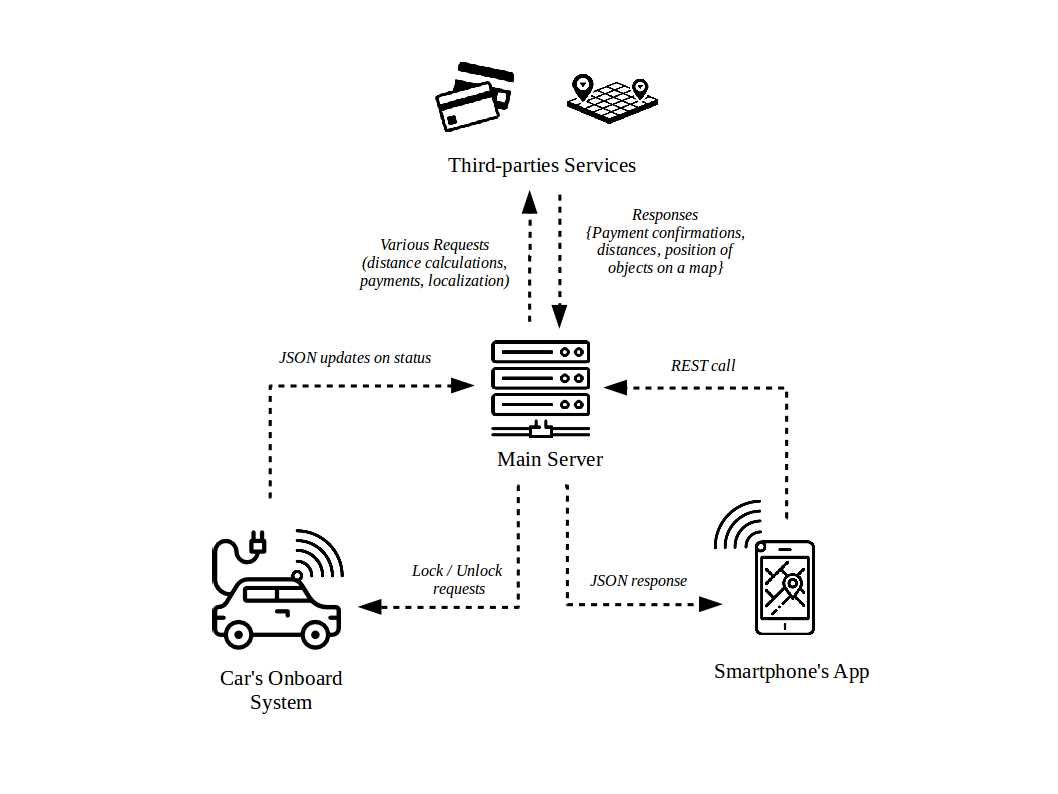
\includegraphics[width=0.88\textwidth]{proposed_system.png}
	\caption{Communication design of the process (anticipating some technology choices we are going to justify in next sections).}
\end{figure}





\subsection{Components Design}

Up to this point we defined the logical components of the system in terms of interfaces and communication protocols. We now proceed with the deploy of the system on the physical nodes identified above, in order to end up with a complete, high-level logical architecture for our system.

\begin{description}
	\item[USER\_MANAGER] \hfill \\
	Considering that all its functionalities are exposed as API by the server to the apps, the component is deployed on the server entirely.
		
	\item[GEOLOCATION] \hfill \\
	Considering that all its functionalities are exposed as API by the server, the component is deployed on the server entirely.

	\item[POSITION] \hfill \\
	This component need the partecipation of both users and cars. Thus the component is deployed on all the three nodes:  user apps, cars and the main server.
	\begin{description}
		\item[POSITION/Users] is deployed as \textbf{USER\_POSITION} on the user apps.
	\end{description}
	
	\item[BOOKING\_MANAGER] \hfill \\
	Considering that all its functionalities are exposed as API by the server, the component is deployed on the server entirely.
	\item[BILLING\_SYSTEM] \hfill \\
	Considering that all its functionalities are exposed as API by the server to the customer's apps, the component is deployed on the server entirely. 

	
	\item[NOTIFIER] \hfill \\
	Considering that its functionality is exposed by the user app, this component is deployed entirely on the user app.
\end{description}

\begin{figure}[H]
	\centering
	\includegraphics[width=0.88\textwidth]{UML/Deploy.png}
	\caption{Graphical visualization of the abstract components needed.}
\end{figure}	

\begin{figure}[H]
	\centering
	\includegraphics[width=1.1\textwidth]{UML/InterfaceDiagram.png}
	\caption{Description of the interfaces of the
 components identified above.}
\end{figure}	

\begin{figure}[H]
	\centering
	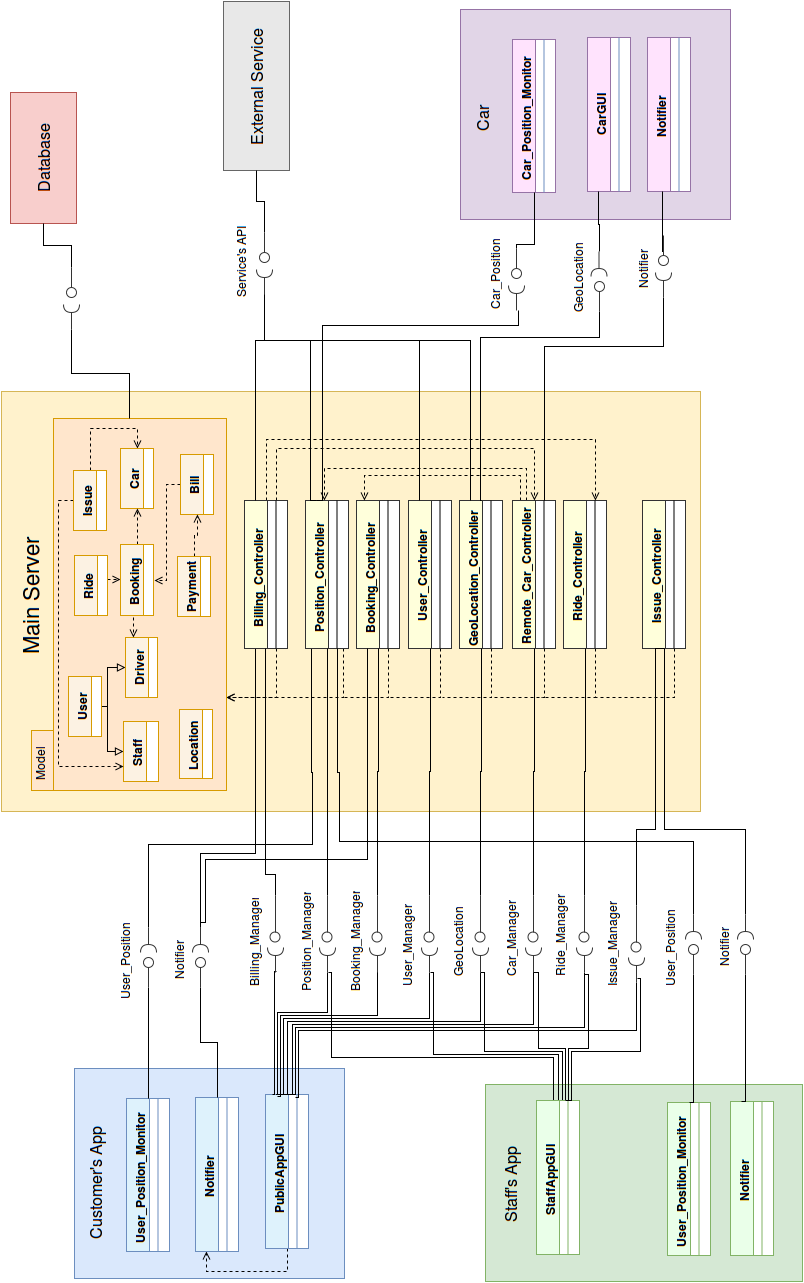
\includegraphics[width=0.88\textwidth]{UML/ComponentsDiagram.png}
	\caption{Components View Diagram of the entire system.}
\end{figure}	

\begin{figure}[H]
	\centering
	\includegraphics[width=0.88\textwidth]{UML/ModelZoomComponents.png}
	\caption{Model zoom of the Components View Diagram.}
\end{figure}	


\newpage
\subsection{Runtime View}

In this section we provide four Sequence Diagram and their description, to ensure the system is coherent.

\subsubsection{Register and Login}
\begin{figure}[H]
	\centering
	\includegraphics[width=1\textwidth]{UML/DDSequenceDiagramLoginReg.png}
	\caption{Sequence Diagram for Registration and Login process of customers.	}
\end{figure}	

\subsubsection{Lookup and Book}
\begin{figure}[H]
	\centering
	\includegraphics[width=1\textwidth]{UML/DDSequenceDiagramBooking.png}
	\caption{Sequence Diagram for Lookup and Booking process of customers.}
\end{figure}

\subsubsection{Ride}
\begin{figure}[H]
	\centering
	\includegraphics[width=1\textwidth]{UML/DDSequenceDiagramRide.png}
	\caption{Sequence Diagram for the Riding process of customers.}
\end{figure}



\subsubsection{Issue Management}
\begin{figure}[H]
	\centering
	\includegraphics[width=0.9\textwidth]{UML/DDSequenceDiagramIssue.png}
	\caption{Sequence Diagram for the Issue Management process for staff operators.}
\end{figure}

In the above diagram we can see how the process of managing issues is carried on by staff operators.

The process share more or less the same workflow as the booking and unlock process for customers, plus some steps related specifically to issues.

It is evident how these additional steps are all managed by ISSUE\_MANAGER alone, as to highlight the single, coherent responsibility we assigned to components.


\subsection{Deployement View}

In order to better understand the technology we chosed to design this deployment diagram, refer to section 2.8: Selected Technologies.

\begin{figure}[H]
	\centering
	\includegraphics[width=0.8\textwidth]{UML/DeployementView.png}
	\caption{Deployement View of the system}
\end{figure}



\subsection{Selected Technologies}


\subsubsection{RESTful API}


\subsubsection{MQTT}


\subsubsection{Nginx}

\subsubsection{PostgreSQL}


\newpage
\section{Algorithm Design}

In this section we define a first sketch of an implementation of BOOKING\_MANAGER. 

Clearly this implementation is extremely naive: it doesn't take care of persisting its status and it doesn't validate the input. However it is effective to show our intention and expectation from the developers.

\hfil\\

\lstinputlisting[language=Python, breaklines=true]{Algo/BookingManager.py}

\newpage
\section{User Interface Design}

\subsection{Mockups}
Mockups have already been included in the RASD (section 3.3: Non Functional Requirements), so they are not being reported here.

\subsection{UX Diagrams}

\begin{figure}[H]
	\centering
	\includegraphics[width=0.88\textwidth]{UML/UXDiagramStaffApp.png}
	\caption{UX Diagram of the interface of staff's application}
\end{figure}	

\begin{figure}[H]
	\centering
	\includegraphics[width=0.88\textwidth]{UML/UXDiagramPublicApp.png}
	\caption{UX Diagram of the interface of customer's application}
\end{figure}

\subsection{BCE Diagrams}

\begin{figure}[H]
	\centering
	\includegraphics[width=1\textwidth]{UML/BCEDiagramStaffApp.png}
	\caption{BCE Diagram of the interface of staff's application}
\end{figure}	
	
\begin{figure}[H]
	\centering
	\includegraphics[width=1\textwidth]{UML/BCEDiagramPublicApp.png}
	\caption{BCE Diagram of the interface of customer's application}
\end{figure}	



\newpage
\section{Conclusions}



\end{document}  
